\chapter{Background}
\todo{back intro}
\section{Fundamentals of Reinforcement Learning}
The term \gls{rl} is used for a wide range of algorithms and methods that learn to make decisions by interacting with an environment. The following will give a brief overview of the most important concepts and terms in \gls{rl}. In particular, this work focuses on model-free, on-policy, policy-optimization algorithms, where the policy used to collect data is the same one being updated. For a thorough treatment of the fundamentals see \cite{SuttonBarto2018}.
\subsection{Markov Decision Processes}
\begin{figure}
\centering
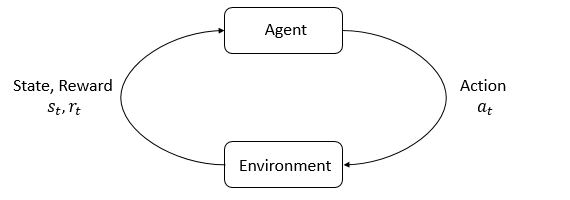
\includegraphics[width=0.8\textwidth]{images/rl_diagram.png}
\caption{TODO   Reinforcement learning framework. The agent interacts with the environment by taking actions and receiving rewards, while the environment transitions to new states based on the agent's actions.}
\label{fig:rl_diagram}
\end{figure}

\gls{rl} is a framework in which an agent learns to make decisions by interacting with its environment.  This interaction is commonly modeled as a \gls{mdp}, defined by the tuple
\[
(\mathcal{S}, \mathcal{A}, P, r, \gamma),
\]
where
\begin{itemize}
  \item \(\mathcal{S}\) is the set of all possible states,
  \item \(\mathcal{A}\) is the set of all possible actions,
  \item \(P(s'\!\mid\!s,a)\) is the probability of transitioning to \(s'\) from \(s\) when taking \(a\),
  \item \(r(s,a)\) is the immediate reward for taking action \(a\) in state \(s\),
  \item \(\gamma\in[0,1)\) is the discount factor, which down‐weights future rewards.
\end{itemize}

At each time step \(t\), the agent interacts with the environment as also shown in Figure~\ref{fig:rl_diagram}. The agent:
\begin{enumerate}
  \item observes \(s_t\),
  \item samples \(a_t\sim\pi_\theta(\cdot\mid s_t)\),
  \item receives \(r_t = r(s_t,a_t)\),
  \item transitions to \(s_{t+1}\sim P(\cdot\mid s_t,a_t)\).
\end{enumerate}
In practice the agent often does not have access to the full state \(s_t\) but only to a partial observation \(o_t\).  We will use the notation interchangeably, i.e.\ \(o_t\) or \(s_t\) depending on the context, unless otherwise specified.
\subsection{Policies}
As already mentioned, the agent's behavior is defined by a policy \(\pi_\theta\), which can be either deterministic or stochastic:
 
    \[
      a_t = \pi_{\theta}(s_t),
    \]
    where \(\pi_{\theta}\) is a deterministic function (e.g., a neural network) mapping state \(s_t\) to action \(a_t\).

    \[
      a_t \sim \pi_{\theta}(\,\cdot\mid s_t),
    \]
    where \(\pi_{\theta}(a\mid s_t)\) is the probability of taking action \(a\) in state \(s_t\).
We parameterize \(\pi_{\theta}\) with \(\theta\) and optimize it to maximize the expected return. Typically, the policy is represented by a neural network taking \(s_t\) as input.

\subsection{Reward and Return}
The agent's goal is to maximize the expected return, which is the total discounted reward over time. 
The reward function \(r_t(s_t,a_t)\) provides immediate feedback to the agent and usually depends on the current state \(s\), action taken by the policy \(a\) and the next state \(s'\). The return \(R_t\) at time step \(t\) is defined as the sum of discounted rewards:
\[
R_t = \sum_{k=0}^{\infty} \gamma^k r_{t+k},
\]
where \(\gamma\) is the discount factor that determines the importance of future rewards. The expected return \(J(\pi)\) is defined as the expected value of the return:

\[
J(\pi) = \mathbb{E}\Bigl[\sum_{t=0}^\infty \gamma^t\,R_t\Bigr].
\]

At every time step \(t\), the agent observes the current state \(s_t\), selects an action \(a_t\) according to a policy \(\pi(a_t\mid s_t)\), receives an immediate reward \(r(s_t,a_t)\), and transitions to the next state \(s_{t+1}\) based on the dynamics \(P\). The goal is to find the optimal policy \(\pi^*\) that maximizes the expected total discounted reward if the agent acts according to it. This formulation can be explicitly stated as the following constrained optimization problem:
\begin{equation}\label{eq:RL_opt}
\begin{aligned}
\text{Find} \quad & \pi^* = \arg\max_{\pi} \mathbb{E}\left[J(\pi)\right] \\
\text{subject to} \quad & s_0 \sim \rho_0, \\
& a_t \sim \pi(\cdot \mid s_t), \quad \forall\ t \in T \\
& s_{t+1} \sim P(\cdot \mid s_t, a_t)
\end{aligned}
\end{equation}

\subsection{Value and Action‐Value Functions}

Given a fixed policy \(\pi_\theta\), we introduce two central quantities that measure the expected return from states and state–action pairs.

\begin{description}
  \item[State‐Value \(V^\pi\):]
    \[
      V^\pi(s)
      = \mathbb{E}\Bigl[\sum_{t=0}^{\infty}\gamma^t\,r_t
      \;\Big|\;s_0 = s\Bigr],
    \]
    the expected total discounted reward when starting in state \(s\) and thereafter following \(\pi_\theta\).
  
  \item[Action‐Value \(Q^\pi\):]
    \[
      Q^\pi(s,a)
      = \mathbb{E}\Bigl[\sum_{t=0}^{\infty}\gamma^t\,r_t
      \;\Big|\;s_0 = s,\;a_0 = a\Bigr],
    \]
    the expected total discounted reward when starting in \(s\), taking action \(a\), then following \(\pi_\theta\).
\end{description}

The Bellman equations decompose each function into reward received until the current state and the discounted value of the next state and action:

\begin{align}
\label{eq:BellmanV}
V^\pi(s)
&= \mathbb{E}_{a\sim\pi(\cdot\mid s)}\bigl[r(s,a)\bigr]
  + \gamma\,\mathbb{E}_{\substack{a\sim\pi(\cdot\mid s)\\s'\sim P(\cdot\mid s,a)}}\bigl[V^\pi(s')\bigr],\\[4pt]
\label{eq:BellmanQ}
Q^\pi(s,a)
&= \mathbb{E}_{s'\sim P(\cdot\mid s,a)}\bigl[r(s,a)\bigr]
  + \gamma\,\mathbb{E}_{\substack{s'\sim P(\cdot\mid s,a)\\a'\sim\pi(\cdot\mid s')}}\bigl[Q^\pi(s',a')\bigr].
\end{align}

The Bellman equations can be combined to give us the advantage function \(A^\pi\), which quantifies the relative value of taking action \(a\) in state \(s\) compared to the average value of the state:
\begin{align}
\label{eq:advantage}
A^\pi(s,a)
&= Q^\pi(s,a) - V^\pi(s)
\end{align}

\subsection{On‐Policy Policy‐Gradient Loop}  
On‐policy methods repeatedly collect fresh data under \(\pi_\theta\) to perform stochastic gradient ascent on \(J(\theta)\) to ultimately improve the policy towards \(\pi^*\). The gradient can be derived from the advantage function \(A^\pi\) as
\begin{align}
\label{eq:policy_gradient}
\nabla_\theta J(\theta)
&= \mathbb{E}\Bigl[\sum_{t=0}^\infty \gamma^t\,\nabla_\theta \log \pi_\theta(a_t\mid s_t)\,A_t\Bigr],
\end{align}
In practice, there are different approaches to approximate the policy gradient \(\nabla_{\theta}J(\theta)\). In the next section, we will focus on the \gls{ppo} algorithm, which is a popular on‐policy method, using a surrogate objective function to optimize the policy.

\subsection{PPO}
\gls{ppo} was introduced by Schulman et al. in \cite{schulman2017proximal}. \gls{ppo} is a family of policy gradient methods that strives for simplicity, efficiency, and robustness. Its central idea is to iteratively improve a stochastic policy by alternating between sampling data from the environment and performing several epochs of first-order optimization on a surrogate objective function. It is an on-policy algorithm.

In \gls{ppo}, actions are sampled from a parameterized probability distribution. For continuous control tasks, the actor typically outputs the parameters of a Gaussian distribution (usually the mean and standard deviation), and actions are sampled as
\[
a_t \sim \mathcal{N}\big(\mu_\theta(s_t),\, \sigma_\theta(s_t)\big).
\]
This stochastic sampling is crucial as it enables the agent to explore a continuous range of actions, thereby promoting both exploration and robustness in learning.

\gls{ppo} builds on the actor-critic framework, where two components are optimized simultaneously. The actor represents the policy \(\pi_\theta\), which selects actions, while the critic estimates a value function \(V_\theta(s)\) that evaluates the quality of states under the current policy. The critic is used to compute an advantage function that quantifies the relative benefit of taking a specific action in a given state. A commonly used method for estimating advantages is \gls{gae}, which effectively reduces variance while introducing a manageable bias that aids learning stability. \gls{gae} computes the advantage as
\[
\hat{A}_t = \sum_{l=0}^{\infty} (\gamma \lambda)^l \delta_{t+l},
\]
with the temporal difference error defined as
\[
\delta_t = r_t + \gamma V_\theta(s_{t+1}) - V_\theta(s_t).
\]
Here, \(r_t\) is the reward received at time \(t\), \(V_\theta(s_t)\) is the estimated value of state \(s_t\) under the current policy, \(\gamma \in [0,1]\) is the discount factor that weighs future rewards, and \(\lambda \in [0,1]\) is a parameter that adjusts the trade-off between bias and variance in the advantage estimates.

A key contribution of \gls{ppo} is the use of a clipped surrogate objective designed to restrict the size of policy updates. Let
\[
r_t(\theta) = \frac{\pi_\theta(a_t \mid s_t)}{\pi_{\theta_{\text{old}}}(a_t \mid s_t)}
\]
denote the probability ratio between the new and the old policies. The clipped surrogate objective is then defined as:
\[
L^{CLIP}(\theta) = \mathbb{E}_t\!\left[\min\!\left(r_t(\theta)\hat{A}_t,\;\text{clip}\left(r_t(\theta),\,1-\epsilon,\,1+\epsilon\right)\hat{A}_t\right)\right],
\]
where \(\hat{A}_t\) is an estimator of the advantage function and \(\epsilon\) is a hyperparameter defining the clipping range. This objective penalizes overly large deviations from the previous policy, ensuring that updates remain conservative while still allowing for meaningful improvements.

In practice, \gls{ppo} combines the policy surrogate loss with additional terms, such as a value function loss and an entropy bonus, yielding a composite objective:
\[
L(\theta) = \mathbb{E}_t \left[ L^{CLIP}_t(\theta) - c_1\, \left(V_\theta(s_t) - V_t^{\text{target}}\right)^2 + c_2\, S\big[\pi_\theta\big](s_t) \right],
\]
where \(c_1\) and \(c_2\) are coefficients that weight the contributions of the value function error and the entropy bonus \(S\big[\pi_\theta\big](s_t)\), respectively. This final objective is optimized using stochastic gradient ascent over multiple epochs on the same batch of on-policy samples.

The overall procedure of \gls{ppo} in an actor-critic setting is summarized in Algorithm~\ref{alg:ppo}. In the algorithm, \(\theta\) denotes the current policy parameters, \(\theta_{\text{old}}\) are the parameters used for generating the on-policy data, \(N\) is the number of parallel actors, \(T\) is the number of timesteps per actor rollout (with \(NT\) total timesteps per batch), \(K\) is the number of epochs over the data, and \(M \le NT\) is the minibatch size.


\begin{algorithm}[H]
\caption{\gls{ppo}, Actor-Critic Style}
\label{alg:ppo}
\begin{algorithmic}[1]
\For{iteration = 1, 2, \dots}
    \For{actor = 1, 2, \dots, N}
        \State Run policy \(\pi_{\theta_{\text{old}}}\) in the environment for \(T\) timesteps.
        \State Compute advantage estimates \(\hat{A}_1, \dots, \hat{A}_T\).
    \EndFor
    \State Optimize the surrogate loss \(L(\theta)\) with respect to \(\theta\) using \(K\) epochs and minibatch size \(M \le NT\).
    \State Update \(\theta_{\text{old}} \leftarrow \theta\).
\EndFor
\end{algorithmic}
\end{algorithm}

Overall, \gls{ppo} strikes a favorable balance between simplicity and performance, making it one of the most widely adopted on-policy algorithms in modern reinforcement learning applications. The following sections will discuss the multi-agent extensions of \gls{ppo} that are used in this work.
\section{Multi-Agent Reinforcement Learning}

This section provides an overview of the theoretical background of \gls{marl} as applied in this work. Our work evaluates both centralized and decentralized training paradigms. In particular, we employ Proximal Policy Optimization (PPO) for centralized training, while also exploring decentralized approaches using Independent PPO (IPPO) and Multi-Agent PPO (MAPPO), which are detailed in subsequent sections.


\section{Multi-Agent Markov Decision Process}
A cooperative multi-agent reinforcement learning problem can be formalized as a \gls{dec-pomdp}\cite{oliehoek_concise_2016}, defined by the tuple
\[
  \bigl(\mathcal{N},\,\mathcal{S},\,\{\mathcal{A}^i\}_{i=1}^N,\,P,\,r,\,\{\Omega^i\}_{i=1}^N,\,O,\,\gamma\bigr)
\]
where:
\begin{itemize}
  \item $\mathcal{N} = \{1,\dots,N\}$ is the set of agents.
  \item $\mathcal{S}$ is the set of global states; $s_0\sim\rho(s)$ is the initial state distribution.
  \item $\mathcal{A}^i$ is the action space of agent $i$, and $\mathcal{A} = \prod_{i=1}^N\mathcal{A}^i$ the joint action space.
  \item $P(s' \mid s, a)$ is the transition kernel, where $a=(a^1,\dots,a^N)\in\mathcal{A}$.
  \item $r(s,a)\in\mathbb{R}$ is the common team reward received by all agents.
  \item $\Omega^i$ is the observation space of agent $i$, and $O(o^1,\dots,o^N\mid s)$ is the joint observation function.
  \item $\gamma\in[0,1)$ is the discount factor.
\end{itemize}
At each time step $t$, each agent $i$ receives a private observation $o^i_t\in\Omega^i$ sampled from $O(\cdot\mid s_t)$ and selects an action $a^i_t\sim\pi^i(a^i\mid\tau^i_t)$ conditioned on its action‐observation history $\tau^i_t$. The joint policy $\pi(a\mid \tau) = \prod_i \pi^i(a^i\mid \tau^i)$ induces an expected discounted return
\[
  J(\pi) \;=\; \mathbb{E}\Bigl[\sum_{t=0}^\infty \gamma^t\,r(s_t, a_t)\Bigr]\,. 
\]

\section{\gls{ppo} in Multi-Agent Settings}
There is two main approaches to applying \gls{ppo} in multi-agent settings: \gls{ippo} and \gls{mappo}. Both approaches extend the single-agent \gls{ppo} algorithm to handle multiple agents, but they differ in how they address the challenges of non-stationarity and credit assignment in multi-agent environments. Their main difference is is wether the critics are centralized or decentralized. In \gls{ippo}, each agent has its own critic, while in \gls{mappo}, a shared critic is used across all agents. This section will provide a brief overview of both approaches.

\subsection{\gls{ippo}}
\gls{ippo} \cite{witt_is_2020} extends the single agent \gls{ppo} (clipped surrogate objective, GAE, value‐loss and entropy bonus) for each agent in isolation, treating the other agents as part of the non‐stationary environment.  Concretely, for each agent \(i\) we optimize
\[
  L_i(\theta_i) \;=\; 
  \mathbb{E}_t \Bigl[\,L^{\mathrm{CLIP}}_i(\theta_i) \;-\; c_1\,\bigl(V_{\phi_i}(o^i_t)-V^{\text{target},\,i}_t\bigr)^2
    \;+\; c_2\,S\bigl[\pi_{\theta_i}\bigr](o^i_t)\Bigr],
\]
where
\[
  L^{\mathrm{CLIP}}_i(\theta_i)
  = \mathbb{E}_t\!\Bigl[\min\bigl(r^i_t(\theta_i)\,\hat A^i_t,\;\mathrm{clip}(r^i_t(\theta_i),1-\epsilon,1+\epsilon)\,\hat A^i_t\bigr)\Bigr],
\]
\(r^i_t(\theta_i)\!=\!\frac{\pi_{\theta_i}(a^i_t\mid o^i_t)}{\pi_{\theta_i}^{\mathrm{old}}(a^i_t\mid o^i_t)}\), and \(\hat A^i_t\) is computed with \gls{gae} using the local critic \(V_{\phi_i}\).  Each agent collects on‐policy rollouts of its own interaction trace \(\{(o^i_t,a^i_t,r_t)\}\) and applies \(K\) epochs of minibatch SGD exactly as in single agent \gls{ppo}.  While this simplicity enables straightforward scaling to many agents, it does not explicitly address the non stationarity introduced by concurrent learning: all stability and performance gains must emerge implicitly from \gls{ppo} conservative updates and entropy regularization.

\subsection{\gls{mappo}}
\gls{mappo} \cite{yu_surprising_2022} retains the \gls{ppo} surrogate and mixed objective but moves to a \gls{ctde} paradigm.  A single policy network \(\pi_\theta(a^i\mid o^i)\) with shared parameters \(\theta\) is used by all agents at execution, while training leverages a centralized critic \(V_\phi(s)\) receiving full state (or joint observations).  The joint optimization target becomes
\[
  L(\theta,\phi) = \mathbb{E}_t\Bigl[\,L^{\mathrm{CLIP}}(\theta)
   \;-\; c_1\bigl(V_\phi(s_t)-V^{\text{target}}_t\bigr)^2
   \;+\; c_2\sum_{i=1}^N S\bigl[\pi_\theta(\cdot\mid o^i_t)\bigr]\Bigr],
\]
where
\[
  L^{\mathrm{CLIP}}(\theta)
  = \mathbb{E}_t\!\Bigl[\min\bigl(r_t(\theta)\,\hat A_t,\;\mathrm{clip}(r_t(\theta),1-\epsilon,1+\epsilon)\,\hat A_t\bigr)\Bigr],
\]
with the joint ratio \(r_t(\theta)=\prod_i \frac{\pi_\theta(a^i_t\mid o^i_t)}{\pi_{\theta_{\text{old}}}(a^i_t\mid o^i_t)}\) or approximated per‐agent, and \(\hat A_t\) estimated via \gls{gae} using the centralized value \(V_\phi\).  By conditioning the critic on the true global state, \gls{mappo} yields lower‐variance advantage estimates and more accurate credit assignment, yet at test time each agent executes only on its local observation \(o^i\), preserving decentralization.  Shared policy parameters encourage coordination and parameter efficient scaling, while the \gls{ctde} split ensures stability through centralized learning.


\section{Quadrotor Control}
The following section provides a brief overview of quadrotor dynamics and control. We will first describe the quadrotor dynamics and how they are commonly modeled in simulation. Finally, we will discuss the classic control methods used for quadrotors with and without payloads.
\begin{figure}
\centering
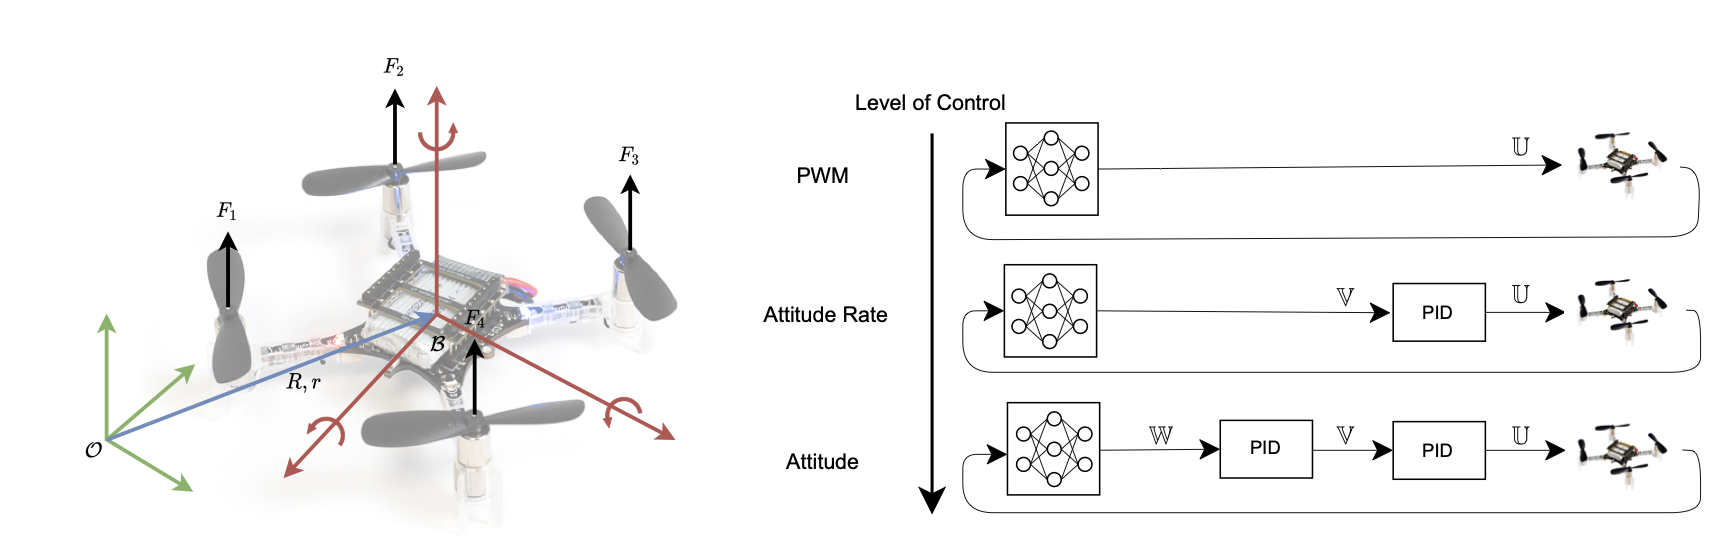
\includegraphics[width=0.8\textwidth]{quadrotor_dynamics.png}
\caption{TODO Quadrotor dynamics and control. The quadrotor is modeled as a rigid body with thrust and torque generated by the rotors. The control inputs are the rotor speeds, which are used to compute the thrust and torques acting on the quadrotor.}
\end{figure}
\subsection{Quadrotor Dynamics}
\subsection{Quadrotor Simulation}
\subsection{Quadrotor Classic Control}
\subsection{Quadrotor With Payloads}

\section{Problem Formulation}

% \section{Quadrotor Control}
% \label{sec:quadrotor_control}

% This section introduces the mathematical model and control design principles for quadrotor UAVs. We begin by defining coordinate frames and state variables, then derive the full nonlinear equations of motion, discuss control allocation and hover linearization, and finally overview classical and learning-based low-level control strategies.

% \subsection{Coordinate Frames and State Representation}
% Let $\{\mathcal I\}$ denote the inertial (world) frame and $\{\mathcal B\}$ the body-fixed frame attached to the quadrotor. The state is
% \[
% \bm x = \bigl(\bm p,\,\bm v,\,R,\,\bm \omega\bigr),
% \]
% where $\bm p\in\mathbb R^3$ is the position of the center of mass in $\{\mathcal I\}$, $\bm v = \dot{\bm p}$ the linear velocity, $R\in \mathrm{SO}(3)$ the rotation matrix from $\{\mathcal B\}$ to $\{\mathcal I\}$, and $\bm\omega\in\mathbb R^3$ the angular velocity in $\{\mathcal B\}$ 
% \todo{cite lee}
% % \cite{lee2010geometric,turn1search11}.

% \subsection{Nonlinear Equations of Motion}
% Denote $m$ the total mass, $I\in\mathbb R^{3\times3}$ the inertia matrix in the body frame, and $g$ the gravitational constant. Each rotor $i$ produces an upward thrust $f_i$ (along $-\bm e_3$ in $\{\mathcal B\}$) and a reaction torque due to drag. Define the total thrust vector in body frame as
% \[
% \bm f = \begin{bmatrix}0\\0\\\sum_{i=1}^4 f_i\end{bmatrix},
% \]
% and the total moment vector
% \[
% \bm\tau
% = \begin{bmatrix}
% l(f_4 - f_2)\\
% l(f_3 - f_1)\\
% \kappa (f_1 - f_2 + f_3 - f_4)
% \end{bmatrix},
% \]
% where $l$ is the arm length and $\kappa$ the drag-to-thrust ratio \cite{turn1search11}.

% The full rigid-body dynamics in the inertial frame are then
% \begin{align}
% m\,\ddot{\bm p}
% &= m\,g\,\bm e_3 + R\,\bm f, \\
% I\,\dot{\bm \omega} + \bm \omega\times I\,\bm \omega
% &= \bm \tau.
% \end{align}

% \subsection{Control Allocation}
% The mapping from rotor inputs $[f_1,\dots,f_4]^\top$ to collective force and moment is linear:
% \[
% \begin{bmatrix}
% F\\M_x\\M_y\\M_z
% \end{bmatrix}
% =
% \begin{bmatrix}
% 1 & 1 & 1 & 1 \\[4pt]
% 0 & -l & 0 & l \\[4pt]
% l & 0 & -l & 0 \\[4pt]
% \kappa & -\kappa & \kappa & -\kappa
% \end{bmatrix}
% \begin{bmatrix}
% f_1\\f_2\\f_3\\f_4
% \end{bmatrix}.
% \]
% Inversion of this allocation matrix yields the required individual rotor thrusts for any desired $(F,M_x,M_y,M_z)$.

% \subsection{Hover Linearization}
% Around the hover equilibrium ($\bm \omega=0$, $R=I$, $f_i = m g/4$), we linearize the translational and rotational dynamics to obtain decoupled second-order systems in $x$, $y$, $z$ and Euler angles. This linear model underpins classical PID and LQR design \cite{mellinger2011minimum}.

% \subsection{Low–Level Control Strategies}
% \paragraph{Classical PID and LQR:}
% Early work employs cascaded PID loops on position, velocity, attitude and angular rate, or LQR on the linearized model for improved performance \cite{mellinger2011minimum}.

% \paragraph{Geometric Nonlinear Control:}
% Geometric tracking controllers on $\mathrm{SE}(3)$ provide almost global stability without coordinate singularities \cite{lee2010geometric}.

% \paragraph{Learned Robust Policies:}
% Recent advances use reinforcement learning (RL) to directly map full state $\bm x$ to rotor commands, yielding low-level policies that transfer from simulation to multiple real quadrotors with domain randomization and noise modeling \cite{molchanov2019sim,turn0search0}. Such policies achieve robust stabilization and trajectory tracking without manual tuning of gains \cite{turn0search3}.



